% =====================================================================
%  Write-up: Laboratorio SOC casero
%  Compilar (desde informe/):  latexmk -pdf main.tex
% =====================================================================
\documentclass[11pt,a4paper,oneside]{report}

% ---------- Idioma y codificación ----------
\usepackage[utf8]{inputenc}
\usepackage[T1]{fontenc}
% babel-spanish (.ldf) no está instalado: se usa el locale .ini de babel.
% Si instalas texlive-lang-spanish puedes volver a \usepackage[spanish,es-tabla]{babel}
\usepackage{babel}
\babelprovide[import,main]{spanish}
\setlocalecaption{spanish}{table}{Tabla}
\setlocalecaption{spanish}{listtable}{Índice de tablas}
\usepackage{lmodern}             % monoespaciada (código) y respaldo
\usepackage{tgtermes}            % texto: TeX Gyre Termes (tipo Times New Roman)
\usepackage[scale=0.92]{tgheros} % títulos: TeX Gyre Heros (tipo Helvetica/Arial)
\usepackage{microtype}

% ---------- Página ----------
\usepackage[margin=2.5cm,headheight=14pt]{geometry}
\usepackage{fancyhdr}
\usepackage{titlesec}
\usepackage{parskip}

% ---------- Figuras y tablas ----------
\usepackage{graphicx}
\graphicspath{{../img/}}
\usepackage{float}
\usepackage{caption}
\usepackage{subcaption}
\usepackage{booktabs}
\usepackage{tabularx}
\usepackage{array}
\usepackage{longtable}

% ---------- Código, colores, cajas ----------
\usepackage{xcolor}
\usepackage{listings}
\usepackage[most]{tcolorbox}
\usepackage{enumitem}

% ---------- Enlaces (siempre al final) ----------
\usepackage{url}
\usepackage[hidelinks]{hyperref}
\hypersetup{pdftitle={Laboratorio SOC casero},pdfauthor={Adolfo Nogués López}}

% =====================================================================
%  Datos del documento (edítalos aquí)
% =====================================================================
\newcommand{\titulo}{Laboratorio SOC desde 0}
\newcommand{\subtitulo}{Despliegue de Wazuh, Suricata y OPNsense sobre KVM\\y análisis de escenarios de ataque}
\newcommand{\autor}{Adolfo Nogués López}
\newcommand{\afiliacion}{Ingeniería Informática -- Universidad de Almería}
\newcommand{\github}{github.com/ualanl248}
\newcommand{\version}{Borrador v0.1}

% =====================================================================
%  Estilo
% =====================================================================
\definecolor{socazul}{HTML}{1F3A5F}
\definecolor{socgris}{HTML}{F4F5F7}
\definecolor{socrojo}{HTML}{B03A2E}
\definecolor{socverde}{HTML}{2E7D4F}
\definecolor{socambar}{HTML}{B7791F}

\titleformat{\chapter}[hang]{\Huge\sffamily\bfseries\color{socazul}}{\thechapter\hspace{12pt}\textcolor{socazul!40}{|}\hspace{12pt}}{0pt}{}
\titlespacing*{\chapter}{0pt}{-20pt}{24pt}
\titleformat{\section}{\Large\sffamily\bfseries\color{socazul}}{\thesection}{1em}{}
\titleformat{\subsection}{\large\sffamily\bfseries\color{socazul!85}}{\thesubsection}{1em}{}

\pagestyle{fancy}
\fancyhf{}
\fancyhead[L]{\small\textcolor{gray}{\titulo}}
\fancyhead[R]{\small\textcolor{gray}{\leftmark}}
\fancyfoot[C]{\thepage}
\renewcommand{\headrulewidth}{0.4pt}
\fancypagestyle{plain}{\fancyhf{}\fancyfoot[C]{\thepage}\renewcommand{\headrulewidth}{0pt}}

\captionsetup{font=small,labelfont={bf,color=socazul}}

% Código (terminal, PowerShell, configuración)
\lstdefinestyle{terminal}{
  basicstyle=\ttfamily\footnotesize,
  backgroundcolor=\color{socgris},
  frame=leftline, framerule=2pt, rulecolor=\color{socazul},
  breaklines=true, breakatwhitespace=false, columns=fullflexible,
  keepspaces=true, showstringspaces=false,
  xleftmargin=8pt, framexleftmargin=6pt, aboveskip=8pt, belowskip=8pt,
  literate={á}{{\'a}}1 {é}{{\'e}}1 {í}{{\'i}}1 {ó}{{\'o}}1 {ú}{{\'u}}1 {ñ}{{\~n}}1
}
\lstset{style=terminal}
% Logs en bruto (JSON de Wazuh, EVE de Suricata, eventos de Windows)
\lstdefinestyle{log}{style=terminal, basicstyle=\ttfamily\scriptsize, rulecolor=\color{socrojo}}
\renewcommand{\lstlistingname}{Listado}
\renewcommand{\lstlistlistingname}{Índice de listados}

% =====================================================================
%  Macros de trabajo
% =====================================================================
% Captura de pantalla:  \captura[ancho]{fichero}{pie de figura}{etiqueta}
\newcommand{\captura}[4][0.9\linewidth]{%
  \begin{figure}[H]\centering
    \fbox{\includegraphics[width=#1,height=0.42\textheight,keepaspectratio]{#2}}
    \caption{#3}\label{fig:#4}
  \end{figure}}

% Caja de "pendiente": aparece en el PDF para que no se olvide nada.
% Para ocultarlas todas en la versión final: \renewcommand{\pendiente}[1]{}
\newtcolorbox{cajapendiente}{colback=socambar!8,colframe=socambar,boxrule=0.6pt,
  left=6pt,right=6pt,top=4pt,bottom=4pt,fonttitle=\bfseries\small,title=Pendiente}
\newcommand{\pendiente}[1]{\begin{cajapendiente}\small #1\end{cajapendiente}}

% Nota / lección aprendida
\newtcolorbox{nota}[1][Nota]{colback=socazul!5,colframe=socazul,boxrule=0.6pt,
  left=6pt,right=6pt,top=4pt,bottom=4pt,fonttitle=\bfseries\small,title=#1}

% Ficha resumen de un escenario de ataque
% \fichaescenario{Técnica MITRE}{Origen}{Objetivo}{Fuente de detección}{Reglas}{Severidad}{Resultado}
\newcommand{\fichaescenario}[7]{%
  \begin{table}[H]\centering\small
  \begin{tabularx}{\linewidth}{>{\bfseries\color{socazul}}l X}
    \toprule
    Técnica MITRE ATT\&CK & #1 \\
    Origen del ataque     & #2 \\
    Objetivo              & #3 \\
    Fuente de detección   & #4 \\
    Reglas / firmas       & #5 \\
    Severidad máxima      & #6 \\
    Resultado             & #7 \\
    \bottomrule
  \end{tabularx}
  \caption{Ficha resumen del escenario}
  \end{table}}

% Hipótesis de detección
\newtcolorbox{hipotesis}{colback=socverde!6,colframe=socverde,boxrule=0.6pt,
  left=6pt,right=6pt,top=4pt,bottom=4pt,fonttitle=\bfseries\small,title=Hipótesis de detección}

% Resultado de cobertura
\newcommand{\si}{\textcolor{socverde}{\textbf{Sí}}}
\newcommand{\no}{\textcolor{socrojo}{\textbf{No}}}
\newcommand{\parcial}{\textcolor{socambar}{\textbf{Parcial}}}
\newcommand{\pend}{\textcolor{gray}{Pendiente}}

% Cronología de un escenario. Uso:
% \begin{cronologia}
%   10:06:20 & windows10 & Wazuh 60122 & Primer fallo de login \\
% \end{cronologia}
\newenvironment{cronologia}
  {\begin{table}[H]\centering\small
   \begin{tabular}{l l l p{0.42\linewidth}}\toprule
   \textbf{Hora} & \textbf{Equipo} & \textbf{Fuente / regla} & \textbf{Evento} \\ \midrule}
  {\bottomrule\end{tabular}\caption{Cronología del escenario}\end{table}}

% =====================================================================
\begin{document}

% ============================ PORTADA ============================
\begin{titlepage}
  \pagecolor{white}\color{black}
  \centering
  \vspace*{3cm}

  {\small\scshape\color{black!70} Write-up técnico}\\[0.6cm]
  {\fontsize{34}{40}\selectfont\bfseries \titulo\par}
  \vspace{0.6cm}
  {\color{black!60}\rule{0.35\linewidth}{1pt}}\\[0.6cm]
  {\Large \subtitulo\par}

  \vfill

  % Imagen de portada opcional (p. ej. la topología):
  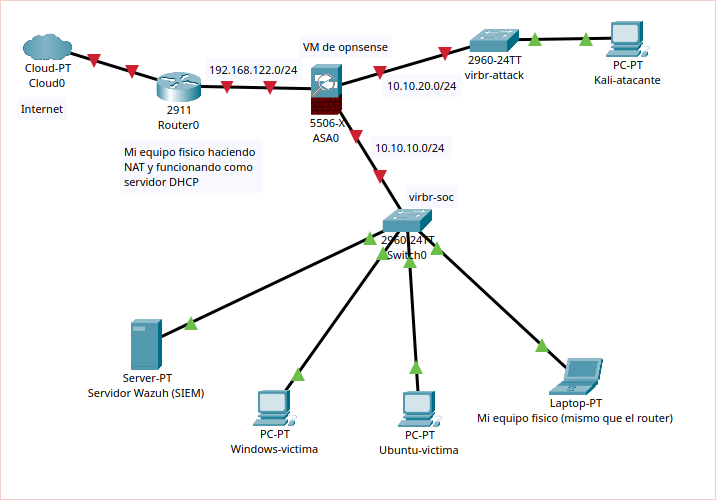
\includegraphics[width=0.7\linewidth]{topologia-fisica}\\[1cm]

  {\Large\bfseries \autor\par}
  \vspace{0.2cm}
  {\large \afiliacion\par}
  \vspace{0.2cm}
  {\ttfamily\color{black!80} \github\par}
  \vspace{1.2cm}
  {\small\color{black!70} \version{} \textbullet{} \today\par}
  \vspace*{1cm}
\end{titlepage}
\nopagecolor\color{black}


\pagenumbering{roman}
% ============================ RESUMEN (TL;DR) ============================
\chapter*{Resumen}
\addcontentsline{toc}{chapter}{Resumen}

Se ha desplegado un laboratorio SOC sobre KVM en un único portátil, con
Wazuh 4.14 como SIEM, OPNsense como cortafuegos entre tres redes
aisladas y Suricata como IDS de red. Hay dos víctimas monitorizadas
(Windows 10 con Sysmon y Ubuntu Server) y una máquina atacante (Kali) en una red
separada, de modo que todo el tráfico del atacante atraviesa el cortafuegos.

Sobre este entorno se han ejecutado escenarios de ataque mapeados a MITRE
ATT\&CK y se ha documentado, para cada uno, la telemetría generada, la regla que
lo detecta, la cronología, la respuesta y los huecos de detección.

Posteriormente se modifican las reglas establecidas y se vuelven a poner a prueba con los mimos ataques. 

El objetivo es conseguir un sistema de monitoreo bien afinado que nos permita tener una visión clara de que sucede en nuestra infraestructura.

\begin{table}[H]\centering\small
\begin{tabularx}{\linewidth}{c X l l}
  \toprule
  \textbf{\#} & \textbf{Escenario} & \textbf{MITRE} & \textbf{Fase} \\
  \midrule
  1  & Escaneo de puertos con nmap (Kali $\rightarrow$ Windows y Ubuntu) & T1046     & Reconocimiento \\
  2  & Escaneo web con nikto (Kali $\rightarrow$ DVWA)                          & T1595.002 & Reconocimiento \\
  3  & Fuerza bruta de rutas con gobuster/dirb (Kali $\rightarrow$ DVWA)        & T1595.003 & Reconocimiento \\
  \addlinespace
  4  & Inyección SQL (Kali $\rightarrow$ DVWA)              & T1190     & Acceso inicial \\
  5  & XSS reflejado (navegador $\rightarrow$ DVWA)                             & T1059.007 & Acceso inicial \\
  6  & Subida de archivo malicioso (Kali $\rightarrow$ DVWA)                    & T1505.003 & Acceso inicial \\
  \addlinespace
  7  & Fuerza bruta SSH con hydra (Kali $\rightarrow$ Ubuntu)                   & T1110     & Acceso a credenciales \\
  8  & Fuerza bruta SSH con hydra (Kali $\rightarrow$ Windows)                  & T1110     & Acceso a credenciales \\
  9  & Fuerza bruta al login web con hydra http-form (Kali $\rightarrow$ DVWA)  & T1110     & Acceso a credenciales \\
  \addlinespace
  10 & Comandos en shell (Ubuntu)                                   & T1059.004 & Ejecución \\
  11 & PowerShell codificado con -EncodedCommand (Windows)                      & T1059.001 & Ejecución \\
  \addlinespace
  12 & Creación de usuario con useradd (Ubuntu)                                 & T1136.001 & Persistencia \\
  13 & Tarea programada con schtasks (Windows)                                  & T1053.005 & Persistencia \\
  14 & Clave de registro Run con reg add (Windows)                              & T1547.001 & Persistencia \\
  \addlinespace
  15 & Borrado del log de seguridad con wevtutil cl (Windows)                   & T1070.001 & Evasión \\
  \addlinespace
  16 & Reverse shell con netcat (Ubuntu $\rightarrow$ Kali)                     & T1059     & Command \& control \\
  \bottomrule
\end{tabularx}
\caption{Escenarios planificados}\label{tab:resumen}
\end{table}
\tableofcontents
\listoffigures
\listoftables
\lstlistoflistings
\cleardoublepage
\pagenumbering{arabic}

% ============================ INTRODUCCIÓN ============================
\chapter{Introducción}\label{cap:introduccion}

\section{Motivación}
Este documento recoge el montaje y la puesta a prueba de un laboratorio SOC
(Security Operations Center) casero, desplegado íntegramente con
máquinas virtuales sobre un portátil con Ubuntu. El objetivo es reproducir a
pequeña escala el trabajo de un analista de nivel 1: recoger telemetría de los
equipos, generar ataques controlados y comprobar si se detectan, cómo se
detectan y qué se puede hacer como respuesta.

\pendiente{Breve explicación de las motivaciones del proyecto}

\section{Objetivos}
\begin{itemize}[leftmargin=*]
  \item Desplegar un SIEM/XDR funcional (Wazuh) en una red aislada.
  \item Segmentar la red con un cortafuegos (OPNsense) y añadir un IDS de red (Suricata).
  \item Monitorizar equipos víctima Windows y Linux con agentes y Sysmon.
  \item Ejecutar escenarios de ataque desde una red de atacante separada (Kali)
        y documentar detección, análisis y respuesta, mapeados a MITRE ATT\&CK.
\end{itemize}

\section{Alcance y limitaciones}
\begin{itemize}[leftmargin=*]
  \item Entorno de laboratorio sin tráfico real de usuarios: el volumen de
        eventos y falsos positivos no es representativo de producción.
  \item Recursos limitados del host (RAM), lo que condiciona cuántas VM pueden
        estar encendidas a la vez.
  \item Todos los ataques se ejecutan contra máquinas propias dentro de redes aisladas.
\end{itemize}

\begin{nota}[Hardware del equipo anfitrión]
\begin{table}[H]\centering\small
\begin{tabularx}{\linewidth}{>{\bfseries\color{socazul}}l X}
  \toprule
  Procesador     & Intel Core i7-8750H @ 2.20\,GHz (6 núcleos / 12 hilos) \\
  Memoria RAM    & 32\,GB DDR4 en dos módulos de 16\,GB
                   (2667\,MT/s) \\
  Almacenamiento & SSD de 234\,GB \\
  Gráfica        & Integrada en el procesador \\
  Hipervisor     & KVM/QEMU con libvirt sobre Ubuntu 26.04 \\
  \bottomrule
\end{tabularx}
\caption{Características del equipo anfitrión}\label{tab:host}
\end{table}
\end{nota}

\section{Herramientas utilizadas}
\begin{table}[H]\centering\small
\begin{tabularx}{\linewidth}{l l X}
  \toprule
  \textbf{Herramienta} & \textbf{Versión} & \textbf{Función en el laboratorio} \\
  \midrule
  KVM / libvirt / virt-manager & --      & Hipervisor y redes virtuales del host \\
  OPNsense                     & 26.7    & Router, cortafuegos, NAT y DHCP entre redes \\
  Suricata (en OPNsense)       & --      & IDS de red sobre la interfaz LAN \\
  Wazuh                        & 4.14    & SIEM/XDR: indexer, manager y dashboard \\
  Sysmon                       & 15.x    & Telemetría avanzada de procesos en Windows \\
  Windows 10 Pro               & 22H2    & Víctima Windows (agente Wazuh + Sysmon) \\
  Ubuntu Server                & 26.04   & Servidor Wazuh y víctima Linux \\
  Kali Linux                   & --      & Máquina atacante en red separada \\
  \bottomrule
\end{tabularx}
\caption{Herramientas y versiones del laboratorio}\label{tab:herramientas}
\end{table}

\section{Estructura del documento}
El capítulo~\ref{cap:arquitectura} describe la arquitectura y las decisiones de
diseño. El capítulo~\ref{cap:despliegue} resume el despliegue y los problemas
encontrados. El capítulo~\ref{cap:escenarios}, núcleo del documento, recoge los
escenarios de ataque con su telemetría, detección, investigación y respuesta.
El capítulo~\ref{cap:cobertura} reúne la cobertura de detección y los ajustes
realizados, y el capítulo~\ref{cap:conclusiones} cierra con lo aprendido. Los
anexos contienen la instalación paso a paso (\ref{anx:instalacion}), los
comandos de gestión (\ref{anx:comandos}) y las configuraciones
(\ref{anx:configuraciones}).

% ============================ ARQUITECTURA ============================
\chapter{Arquitectura y decisiones de diseño}\label{cap:arquitectura}

\section{Topología}
El laboratorio se compone de tres redes virtuales de libvirt. La red
default (NAT del host) hace de Internet para OPNsense. La red
soc-lab es la LAN interna donde se encuentran el SIEM y las víctimas. Y la red attack aísla a la máquina atacante.

\captura{topologia-fisica}{Topología del laboratorio (modelada en Packet Tracer)}{topologia}

\begin{table}[H]\centering\small
\begin{tabularx}{\linewidth}{l l l X}
  \toprule
  \textbf{Red libvirt} & \textbf{Puente} & \textbf{Subred} & \textbf{Uso} \\
  \midrule
  default & virbr0       & 192.168.122.0/24 & WAN de OPNsense (NAT + DHCP de libvirt) \\
  soc-lab & virbr-soc    & 10.10.10.0/24    & LAN: SIEM y víctimas \\
  attack  & virbr-attack & 10.10.20.0/24    & Red del atacante (Kali) \\
  \bottomrule
\end{tabularx}
\caption{Redes virtuales del laboratorio}\label{tab:redes}
\end{table}

\begin{table}[H]\centering\small
\begin{tabularx}{\linewidth}{l l c c c X}
  \toprule
  \textbf{VM} & \textbf{IP} & \textbf{RAM} & \textbf{vCPU} & \textbf{Disco} & \textbf{Rol} \\
  \midrule
  opnsense       & 10.10.10.1 / 10.10.20.1 & 2 GB & 2 & 20 GB & Router, firewall, DHCP, Suricata \\
  wazuh          & 10.10.10.10             & 8 GB & 4 & 50 GB & SIEM \\
  windows10      & 10.10.10.130 (DHCP)     & 4 GB & 2 & 50 GB & Víctima Windows con Sysmon y agente \\
  ubuntu-victima & 10.10.10.20             & 2 GB & 1 & 15 GB & Víctima Linux con agente \\
  kali           & 10.10.20.10             & 4GB   & 2 & 80GB   & Atacante \\
  host           & 10.10.10.254            & --   & -- & --   & Administración y acceso al dashboard \\
  \bottomrule
\end{tabularx}
\caption{Inventario de máquinas virtuales}\label{tab:inventario}
\end{table}

\section{Flujo de la telemetría}
\begin{itemize}[leftmargin=*,itemsep=0pt]
  \item Endpoint Windows: registro de seguridad y Sysmon $\rightarrow$ agente Wazuh $\rightarrow$ manager (10.10.10.10).
  \item Endpoint Linux: auth.log, syslog $\rightarrow$ agente Wazuh $\rightarrow$ manager.
  \item Red: Suricata en la LAN de OPNsense $\rightarrow$ eve.json $\rightarrow$ agente Wazuh de OPNsense $\rightarrow$ manager.
\end{itemize}



% ============================ DESPLIEGUE ============================
\chapter{Despliegue}\label{cap:despliegue}

Este capítulo resume el despliegue y se centra en lo que no está en la
documentación oficial. El paso a paso completo, con todas las capturas, está en
el anexo~\ref{anx:instalacion}.

\section{Resumen de las configuraciones}
\begin{table}[H]\centering\small
\begin{tabularx}{\linewidth}{l X l}
  \toprule
  \textbf{Componente} & \textbf{Configuración relevante} & \textbf{Detalle} \\
  \midrule
  OPNsense & WAN vtnet0 (DHCP), LAN vtnet1 10.10.10.1/24, DHCP .100--.200, interfaz ATTACK 10.10.20.1/24 & \ref{sec:a-opnsense} \\
  Wazuh    & All-in-one 4.14, IP estática 10.10.10.10 & \ref{sec:a-wazuh} \\
  Windows 10 & Usuario local Victima, Sysmon, OpenSSH Server, agente Wazuh & \ref{sec:a-windows} \\
  Suricata & IDS (PCAP live) en LAN, promiscuo; rulesets abuse.ch y ET open; plugin os-wazuh-agent & \ref{sec:a-suricata} \\
  Ubuntu víctima & IP estática 10.10.10.20, agente Wazuh & \ref{sec:a-ubuntu} \\
  Kali & Red attack, 10.10.20.10, puerta de enlace OPNsense & \ref{sec:a-kali} \\
  \bottomrule
\end{tabularx}
\caption{Resumen del despliegue}\label{tab:despliegue}
\end{table}

\captura{wazuh-agentes}{Estado final: agentes de Windows, OPNsense y Ubuntu registrados en Wazuh}{wazuh-agentes}

\section{Conjuntos de reglas de Suricata}
\begin{itemize}[leftmargin=*,itemsep=0pt]
  \item Reputación / listas negras:
        abuse.ch SSL Fingerprint Blacklist, abuse.ch SSL IP Blacklist,
        abuse.ch ThreatFox, abuse.ch URLhaus; ET open botcc,
        ET open compromised y ET open drop.
  \item Detección de ataques:
        ET open emerging-attack\_response, emerging-scan,
        emerging-exploit, emerging-malware, emerging-policy,
        emerging-dns y emerging-web\_client.
  \item Excluidos explícitamente:
        emerging-info y emerging-hunting, por generar un volumen
        elevado de alertas sobre actividad legítima.
  \item Configuración del motor:
        modo IDS (PCAP live, sin bloqueo) sobre la interfaz LAN;
        HOME\_NET restringido a 10.10.10.0/24, de modo
        que la red atacante (10.10.20.0/24), la WAN e Internet
        se consideran externas; actualización diaria de reglas
        programada.
  \item Validación:
        firma SID 2100498 (GPL ATTACK\_RESPONSE id check returned
        root), disparada sirviendo la cadena uid=0(root) desde
        un servidor HTTP en el lado WAN (192.168.122.1:8000),
        ya que el dominio de prueba testmynids.org ha caducado. La alerta
        se recibe en Wazuh mediante el agente de OPNsense
        (regla 86601).
  \item Ajuste necesario:
        desactivar la descarga de hardware (CRC, TSO y LRO) en las
        interfaces de OPNsense; con las tarjetas virtio, Suricata no
        generaba alertas hasta aplicar este cambio.
\end{itemize}

\section{Instantáneas}
\begin{table}[H]\centering\small
\begin{tabularx}{\linewidth}{l l X}
  \toprule
  \textbf{VM} & \textbf{Instantánea} & \textbf{Estado} \\
  \midrule
  opnsense  & opnsense-base         & Instalado y configurado \\
  wazuh     & wazuh-base            & Wazuh 4.14 instalado y funcionando \\
  windows10 & windows-limpio        & Windows recién instalado \\
  windows10 & windows-monitorizado  & Sysmon y agente Wazuh funcionando \\
  \bottomrule
\end{tabularx}
\caption{Instantáneas de las máquinas virtuales}\label{tab:snapshots}
\end{table}

% ===================== ESCENARIOS DE ATAQUE Y RESPUESTA =====================
\chapter{Escenarios de ataque y respuesta}\label{cap:escenarios}


% ============================ COBERTURA Y AFINADO ============================
%\chapter{Cobertura de detección y afinado}\label{cap:cobertura}


% ============================ CONCLUSIONES ============================
%\chapter{Conclusiones}\label{cap:conclusiones}




% ---------- Bibliografía ----------
\cleardoublepage
\phantomsection
\addcontentsline{toc}{chapter}{Bibliografía}
\nocite{*}   % muestra todas las entradas del .bib; quítalo para mostrar solo las citadas
\bibliographystyle{unsrt}
\bibliography{bibliografia}

% ---------- Anexos ----------
\appendix
% ================= ANEXO A: INSTALACIÓN PASO A PASO =================
\chapter{Instalación paso a paso}\label{anx:instalacion}

Este anexo recoge el proceso completo de instalación con todas las capturas,
como referencia para reproducir el laboratorio. El resumen y las decisiones
están en los capítulos~\ref{cap:arquitectura} y~\ref{cap:despliegue}.

\captura[0.75\linewidth]{esquema-red}{Esquema lógico de las redes y del direccionamiento}{esquema-red}

\section{Preparación del host: KVM y redes virtuales}\label{sec:a-host}
Se instala KVM con libvirt y virt-manager en el Ubuntu anfitrión y se crea la
red aislada soc-lab.

\captura[0.6\linewidth]{redes-libvirt}{Redes virtuales activas en libvirt}{redes-libvirt}

\pendiente{Añade el XML o los comandos con los que creaste la red soc-lab.}

% ---------------------------------------------------------------------
\section{OPNsense: router y cortafuegos}\label{sec:a-opnsense}
OPNsense se instala con dos interfaces VirtIO: vtnet0 como WAN en la
red default y vtnet1 como LAN en soc-lab.

\captura{virt-install-opnsense}{Creación de la VM de OPNsense con virt-install}{virt-opnsense}
\captura[0.6\linewidth]{opnsense-menu-instalacion}{Instalador de OPNsense 26.7 (UFS)}{opn-menu}
\captura[0.6\linewidth]{opnsense-aviso-ram}{Aviso del instalador por RAM inferior a 3 GB}{opn-ram}
\captura[0.6\linewidth]{opnsense-progreso}{Progreso de la instalación}{opn-progreso}
\captura{opnsense-interfaces}{Asignación de interfaces WAN y LAN}{opn-if}
\captura{opnsense-lan-dhcp}{Configuración de la LAN (10.10.10.1/24) y del servidor DHCP (.100--.200)}{opn-lan}
\captura[0.7\linewidth]{opnsense-resumen-ips}{Resumen de direcciones de OPNsense}{opn-resumen}
\captura{snapshot-opnsense}{Instantánea opnsense-base tras la configuración}{snap-opn}

% ---------------------------------------------------------------------
\section{Wazuh: servidor SIEM}\label{sec:a-wazuh}
Wazuh 4.14 se despliega en modo all-in-one sobre Ubuntu Server con IP
estática 10.10.10.10.

\begin{lstlisting}[language=bash,caption={Creación de la VM de Wazuh},label=lst:virt-wazuh]
virt-install --connect qemu:///system \
  --name wazuh --memory 8192 --vcpus 4 \
  --disk size=50,bus=virtio \
  --cdrom /var/lib/libvirt/images/ubuntu-26.04.1-live-server-amd64.iso \
  --network network=soc-lab,model=virtio \
  --osinfo detect=on,require=off \
  --graphics spice --noautoconsole
\end{lstlisting}

\captura[0.6\linewidth]{wazuh-ip-estatica}{Configuración de red estática del servidor Wazuh}{wazuh-ip}

\begin{lstlisting}[language=bash,caption={Instalación all-in-one de Wazuh},label=lst:wazuh-install]
curl -sO https://packages.wazuh.com/4.14/wazuh-install.sh
sudo bash ./wazuh-install.sh -a -i
\end{lstlisting}

\captura{wazuh-install-script}{Lanzamiento del instalador de Wazuh}{wazuh-script}
\captura{snapshot-wazuh}{Instantánea wazuh-base con Wazuh funcionando}{snap-wazuh}

\begin{nota}[Seguridad]
El instalador muestra la contraseña del usuario admin del dashboard en
claro. No se incluye esa captura en el documento; si se añade, debe pixelarse
antes.
\end{nota}

% ---------------------------------------------------------------------
\section{Víctima Windows 10: Sysmon y agente Wazuh}\label{sec:a-windows}

\begin{lstlisting}[language=bash,caption={Creación de la VM Windows 10},label=lst:virt-win]
virt-install --connect qemu:///system \
  --name windows10 --memory 4096 --vcpus 2 \
  --disk size=50,bus=sata \
  --cdrom /var/lib/libvirt/images/Win10_22H2_EnglishInternational_x64v1.iso \
  --network network=soc-lab,model=e1000e \
  --osinfo win10 --graphics spice --noautoconsole
virt-viewer -c qemu:///system --reconnect windows10 &
\end{lstlisting}

\captura[0.6\linewidth]{windows-instalando}{Instalación de Windows 10 Pro}{win-instalando}
\captura[0.6\linewidth]{windows-usuario-victima}{Creación del usuario local Victima}{win-usuario}
\captura{windows-ipconfig-ping}{Windows obtiene IP por DHCP de OPNsense y sale a Internet}{win-ip}
\captura{snapshot-windows-limpio}{Instantánea windows-limpio}{snap-win-limpio}

\subsection{Sysmon}
Sysmon se instala con la configuración de SwiftOnSecurity~\cite{swiftonsecurity}.

\begin{lstlisting}[caption={Instalación de Sysmon (PowerShell como administrador)},label=lst:sysmon]
cd $env:TEMP
Invoke-WebRequest https://download.sysinternals.com/files/Sysmon.zip -OutFile Sysmon.zip
Expand-Archive Sysmon.zip -DestinationPath Sysmon -Force
Invoke-WebRequest https://raw.githubusercontent.com/SwiftOnSecurity/sysmon-config/master/sysmonconfig-export.xml -OutFile sysmonconfig.xml
.\Sysmon\Sysmon64.exe -accepteula -i sysmonconfig.xml
\end{lstlisting}

\captura{sysmon-instalacion}{Instalación de Sysmon}{sysmon-inst}
\captura{sysmon-servicio}{Servicio Sysmon64 en ejecución y primeros eventos}{sysmon-svc}
\captura{sysmon-evento}{Evento Sysmon ID~1 (creación de proceso) en detalle}{sysmon-ev}

\subsection{OpenSSH Server}
Se habilita OpenSSH en Windows para disponer de una superficie de ataque
remota (escenario~\ref{sec:esc-bruteforce}).

\captura{windows-openssh}{Instalación y arranque de OpenSSH Server con PowerShell como shell por defecto}{win-ssh}

\subsection{Agente Wazuh}
\begin{lstlisting}[caption={Instalación del agente Wazuh en Windows},label=lst:agente-win]
Invoke-WebRequest -Uri https://packages.wazuh.com/4.x/windows/wazuh-agent-4.14.9-1.msi `
  -OutFile $env:tmp\wazuh-agent
msiexec.exe /i $env:tmp\wazuh-agent /q WAZUH_MANAGER='10.10.10.10' WAZUH_AGENT_NAME='windows10'
NET START Wazuh
\end{lstlisting}

\captura{wazuh-agente-windows}{Agente Wazuh instalado y arrancado}{agente-win}
\captura{snapshot-windows-monitorizado}{Instantánea windows-monitorizado}{snap-win-mon}

\pendiente{Añade cómo se ingesta el canal de Sysmon en el agente
(ossec.conf, Microsoft-Windows-Sysmon/Operational) si lo configuraste.}

% ---------------------------------------------------------------------
\section{Suricata en OPNsense e integración con Wazuh}\label{sec:a-suricata}
Suricata se activa en modo IDS (PCAP live) sobre la interfaz LAN, en modo
promiscuo, con los siguientes conjuntos de reglas:

\begin{itemize}[leftmargin=*,itemsep=0pt]
  \item Reputación / listas negras: abuse.ch SSL Fingerprint Blacklist,
        SSL IP Blacklist, ThreatFox, URLhaus; ET open botcc,
        compromised y drop.
  \item Detección de ataques: ET open emerging-attack\_response
        (imprescindible para la prueba de testmynids.org),
        emerging-scan, emerging-exploit, emerging-malware,
        emerging-policy, emerging-dns y emerging-web\_client.
\end{itemize}

\captura[0.7\linewidth]{suricata-ajustes}{Ajustes generales de Suricata en OPNsense}{suri-ajustes}
\captura[0.6\linewidth]{suricata-rulesets}{Selección de rulesets}{suri-rulesets}
\captura[0.6\linewidth]{suricata-reglas}{Reglas cargadas tras descargar los conjuntos}{suri-reglas}

Para que las alertas de Suricata lleguen al SIEM se instala el plugin
os-wazuh-agent en OPNsense.

\captura[0.7\linewidth]{opnsense-wazuh-agent}{Instalación del plugin os-wazuh-agent}{opn-agent}

% ---------------------------------------------------------------------
\section{Víctima Linux: Ubuntu Server}\label{sec:a-ubuntu}
\begin{lstlisting}[language=bash,caption={Creación de la VM ubuntu-victima},label=lst:virt-ubu]
virt-install --connect qemu:///system \
  --name ubuntu-victima --memory 2048 --vcpus 1 \
  --disk size=15,bus=virtio \
  --cdrom /var/lib/libvirt/images/ubuntu-26.04.1-live-server-amd64.iso \
  --network network=soc-lab,model=virtio \
  --osinfo detect=on,require=off --graphics spice --noautoconsole
\end{lstlisting}

\captura[0.6\linewidth]{ubuntu-victima-ip}{IP estática 10.10.10.20 en ubuntu-victima}{ubu-ip}

\pendiente{Documenta la instalación del agente Wazuh en ubuntu-victima.}

% ---------------------------------------------------------------------
\section{Red de ataque y Kali Linux}\label{sec:a-kali}
La máquina atacante se coloca en una red propia (attack, 10.10.20.0/24)
conectada a una tercera interfaz de OPNsense, para que todo su tráfico hacia
las víctimas pase por el cortafuegos y por Suricata.

\begin{lstlisting}[language=bash,caption={Definición de la red attack},label=lst:red-attack]
cat > attack.xml <<'EOF'
<network>
  <name>attack</name>
  <bridge name="virbr-attack"/>
</network>
EOF
virsh -c qemu:///system net-define attack.xml
virsh -c qemu:///system net-autostart attack
virsh -c qemu:///system net-start attack
\end{lstlisting}

\captura[0.6\linewidth]{red-attack}{Creación de la red attack}{red-attack}
\captura[0.7\linewidth]{firewall-attack}{Regla de cortafuegos para la red ATTACK en OPNsense}{fw-attack}

\begin{lstlisting}[language=bash,caption={Configuración de red estática en Kali},label=lst:kali-red]
sudo nmcli con mod "Wired connection 1" ipv4.method manual \
  ipv4.addresses 10.10.20.10/24 ipv4.gateway 10.10.20.1 ipv4.dns 10.10.20.1
sudo nmcli con up "Wired connection 1"
\end{lstlisting}

\captura{kali-red}{Configuración de red en Kali}{kali-red}
\captura[0.6\linewidth]{kali-ping}{Kali alcanza su puerta de enlace e Internet a través de OPNsense}{kali-ping}

\pendiente{La regla actual permite todo el tráfico desde ATTACK. Decide y documenta
qué tráfico se permite hacia la LAN para cada escenario.}


% ============================ ANEXO B: COMANDOS ============================
\chapter{Comandos de gestión del laboratorio}\label{anx:comandos}

\begin{lstlisting}[language=bash,caption={Gestión de VM con virsh},label=lst:virsh]
# Arrancar máquinas
virsh -c qemu:///system start opnsense
virsh -c qemu:///system start windows10

# Ver máquinas encendidas y apagadas
virsh -c qemu:///system list --all

# Abrir visor gráfico
virt-viewer -c qemu:///system --reconnect windows10 &

# Crear instantánea
virsh -c qemu:///system snapshot-create-as windows10 windows-monitorizado \
  "Sysmon + agente Wazuh funcionando"

# Borrar instantánea
virsh -c qemu:///system snapshot-delete windows10 windows-limpio
\end{lstlisting}

% ================= ANEXO C: CONFIGURACIONES =================
\chapter{Configuraciones}\label{anx:configuraciones}

Los ficheros completos están en la carpeta configs/ del repositorio.
Aquí se incluyen solo los fragmentos relevantes.

\section{Red attack de libvirt}
\lstinputlisting[language=XML,caption={configs/libvirt/attack.xml},label=lst:cfg-attack]{../configs/libvirt/attack.xml}

\section{Agente Wazuh en Windows}
\pendiente{Fragmento de ossec.conf con el localfile del canal
Microsoft-Windows-Sysmon/Operational.}

\section{Reglas locales de Wazuh}
\pendiente{Contenido de local\_rules.xml cuando crees reglas propias.}


\end{document}
